\exer{[INT-002]}
\setcounter{numques}{0}~\\


\question{}

\begin{lstlisting}
a=0
b=1
n=100
h=(b-a)/n
x=a
somme=f(a)
for k in range(1,n) :
    x=x+h
    somme=somme+f(x)
print(somme*h)

\end{lstlisting}

\question{} 

\begin{lstlisting}
def rect_gauche(f,a,b,n):
    h=(b-a)/n
    x=a
    somme=f(a)
    for k in range(1,n) :
        x=x+h
        somme=somme+f(x)
    return somme*h

\end{lstlisting}

\question{}


\begin{lstlisting}
def rect_droit(f,a,b,n):
    h=(b-a)/n
    x=a+h
    somme=f(x)
    for k in range(1,n) :
        x=x+h
        somme=somme+f(x)
    return somme*h

\end{lstlisting}

\question{} 

\begin{lstlisting}
def f(x):
    return 4/(1+x**2)
\end{lstlisting}

\question{}


\begin{minipage}{0.5\textwidth}
\begin{lstlisting}
liste_n=[5,10,100,1000,10000,int(1E5)]
yrd=[rect_droit(f,0,1,n) for n in liste_n]
yrg=[rect_gauche(f,0,1,n) for n in liste_n]

plt.clf()
plt.semilogx(liste_n,yrg,'b*',label='Méthode des rectangle à gauche')
plt.semilogx(liste_n,yrd,'r*',label='Méthode des rectangle à droite')
plt.legend()
plt.grid()
plt.xlabel('n')
plt.ylabel('Estimation de $\\int_0^1\\frac{4dx}{1+x^2}$')
plt.savefig('tp10_q5_durif.png')
\end{lstlisting}
\end{minipage}
\begin{minipage}{0.5\textwidth}
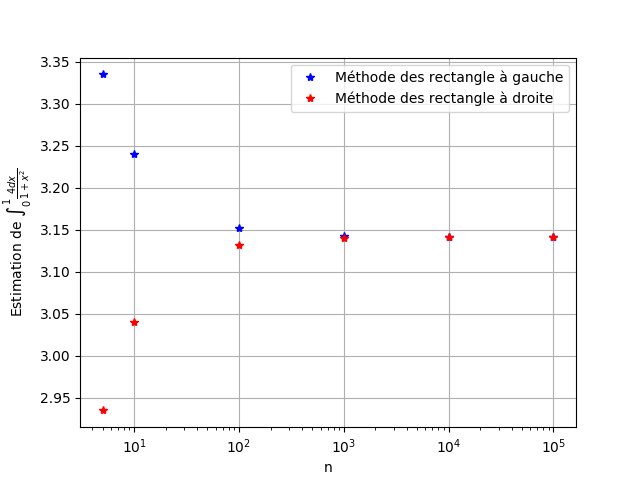
\includegraphics[width=0.9\textwidth]{tp10_q5_durif.png}
\end{minipage}



\question{}




\question{} 

\begin{lstlisting}
def calcul_in(n):
    return rect_gauche(lambda x:x/(1+x**n),a,b,100)
\end{lstlisting}

\question{} 

\begin{minipage}{0.5\textwidth}
\begin{lstlisting}
liste_n=[1,2,4,7,10,100,1000]
y=[calcul_in(n) for n in liste_n]

plt.clf()
plt.plot(liste_n,y,'b*')
plt.xlabel('n')
plt.ylabel('Estimation de $\\int_0^1\\frac{dx}{1+x^n}$')
plt.grid()
plt.savefig('tp10_q8_durif.png')
\end{lstlisting}
\end{minipage}
\begin{minipage}{0.5\textwidth}
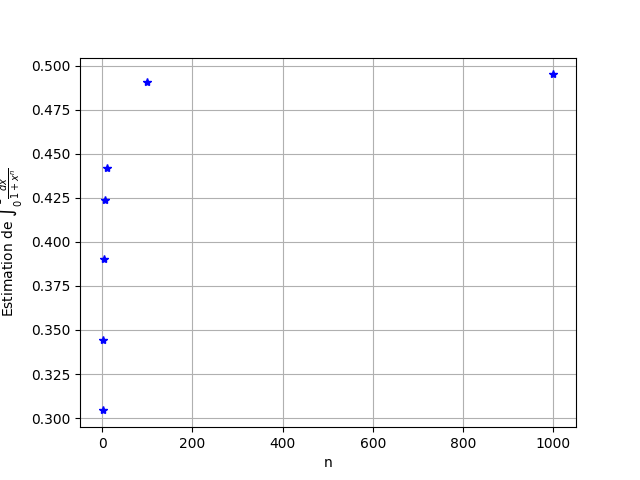
\includegraphics[width=0.9\textwidth]{tp10_q8_durif.png}
\end{minipage}